%%%%%%%%%%%%%%%%%%%%%%%%%
% Dokumentinformationen %
%%%%%%%%%%%%%%%%%%%%%%%%%
\newcommand{\titleinfo}{Volkswirtschaftslehre}
\newcommand{\authorname}{\href{mailto:michel.gisler@hsr.ch}{M. Gisler}}
\newcommand{\authoremail}{\href{mailto:michel.gisler@hsr.ch}{M. Gisler} }
\newcommand{\versioninfo}{$ V1.0 $}

%%%%%%%%%%%%%%%%%%%%%%%%%%%%%%%%%%%%%%%%%%%%%
% Standard projektübergreifender Header für 
% - Makros 
% - Farben
% - Mathematische Operatoren
%
% dORT NUR ERGÄNZEN, NICHTS LÖSCHEN
%%%%%%%%%%%%%%%%%%%%%%%%%%%%%%%%%%%%%%%%%%%%%
%BuG-Fix
%Package pdf Error: Driver file ................ not found
%If you have a luatex driver fail uncomment these lines
\RequirePackage{luatex85}
\def\pgfsysdriver{pgfsys-pdftex.def}

% Genereller Header
\documentclass[11pt,twoside,a4paper,fleqn]{article}
% Dateiencoding
\usepackage[utf8]{inputenc}
\usepackage[T1]{fontenc}	%ä,ü...
% Seitenränder
\usepackage[left=1.27cm,right=1.27cm,top=1cm,bottom=1cm,includeheadfoot]{geometry}
% Sprachpaket 
\usepackage[english, ngerman]{babel} % Silbentrennung und Rechtschreibung Englisch und Deutsch

%%%%%%%%%%%%%%%%%%%%%%%
%% Wichtige Packages %%
%%%%%%%%%%%%%%%%%%%%%%%
\usepackage{amsmath}                % Allgemeine Matheumgebungen									
\usepackage{amssymb}                % Fonts: msam,msbm, eufm & Mathesymbole, Mengen (lädt automatisch amsfonts)									
\usepackage{array}                  % \newcolumntype, \firsthline, ,\lasthline, m{width}, b{width}									
\usepackage{caption}                % Bildunterschriften									
\usepackage{enumitem}               % basic environments: enumerate, itemize, description									
\usepackage{fancybox}               % \fbox: \shad­ow­box, \dou­ble­box, \oval­box, \Oval­box									
\usepackage{fancyhdr}               % Seiten schöner gestalten, insbesondere Kopf- und Fußzeile									
\usepackage{floatflt}               % Textumflossene Abbildungen \begin{floatingfigure}[r]{Breite} : r rechts, l links, p links auf geraden Seiten und rechts auf ungeraden Seiten								
\usepackage{graphicx}               % \includegraphics[keyvals]{imagefile}, [draft]graphicx zeigt nur Namen und Rahmen an, [final] hebt diese option auf => Bild wird angezeigt    									
\usepackage{hyperref}               % Erstellt Verweise innerhalb und nach außerhalb eines PDF Dokumentes.									
\usepackage{lastpage}               % Bspw. : Page 1 of 3 => \thepage\ of \pageref{LastPage}									
\usepackage{listings}               % Erlaubt es Programmcode in der gewünschten Sprache zu hinterlegen (C++, Matlab,..). Definition der Sprache mit \lstset{language=name}..									
\usepackage{longtable}              % Longtable erlaubt es Tabellen zu erstellen die bei der nächsten Seite weiterlaufen. (Bricht automatisch um)									
\usepackage{mathabx}                % Mathesymbole									
\usepackage{mathrsfs}               % \mathscr (Benötigt für Fourierreihen-Symbol)									
%\usepackage{mathtools}              % Extension package to amsmath									
\usepackage{multicol}               % multicols-Umgebung \begin{multicols}{3} erzeugt Abschnitt mit 3 Spalten									
\usepackage{multirow}               % Tabelle: ermöglicht es Felder mehrerer Zeilen in einem zusammenzufassen									
\usepackage{pdflscape}              % adds PDF support to the environment 'landscape'									
\usepackage{pxfonts}                % Symbole, griechisches Alphabet, Integrale...									
\usepackage{rotating}               % sideways, turn{degree}, rotate{degree}, sidewaysfigure, sidewaystable Umgebung									
\usepackage{subcaption}             % Bildunterschriften für Subfigures									
\usepackage{tabularx}               % tabularx-Umgebung: Hat feste Gesamtbreite, \begin{tabularx}{\textwidth}{c c c c c} X: Spalte mit variabler Breite, l, c, r, p{breite}, m{breite}									
\usepackage{textcomp}               % text symbols: baht, bullet, copyright, musical-note, onequarter, section, yen									
\usepackage{tikz}                   % Tikz Umgebung zur Grafikerzeugung									
\usepackage{titlesec}               % Überschriften zu Textabstände
\usepackage{trfsigns}               % Transformationszeichen \laplace, \Laplace..									
\usepackage{trsym}                  % Weitere Laplace Zeichen erlaubt auch vertikale Transformationszeichen									
\usepackage{verbatim}               % verbatim, verbatim*, comment Umgebung									
\usepackage{wrapfig}                % Textumflossene Bilder und Tabellen, \begin{wrapfigure}[Zeilen]{Position}[Ueberhang]{Breite}									
\usepackage{xcolor}                 % \pagecolor{color}, \textcolor{color}{text}, \colorbox{color}{text}, \fcolorbox{border-color}{fill-color}{text}									
\usepackage{titlesec}
% Zum Bilder einfach in Tabellen einfügen (valign=t)
\usepackage[export]{adjustbox}

%%%%%%%%%%%%%%%%%%%%
% Generelle Makros %
%%%%%%%%%%%%%%%%%%%%
\newcommand{\skript}[1]{$_{\textcolor{red}{\mbox{\small{Skript S.#1}}}}$}
\newcommand{\verweis}[2]{\small{(siehe auch \ref{#1}, #2 (S. \pageref{#1}))}}
\newcommand{\verweiskurz}[1]{(\small{siehe \ref{#1}\normalsize)}}
\newcommand{\subsubadd}[1]{\textcolor{black}{\mbox{#1}}}
\newcommand{\formelbuch}[1]{$_{\textcolor{red}{\mbox{\small{S#1}}}}$}

\newcommand{\kuchling}[1]{$_{\textcolor{red}{\mbox{\small{Kuchling #1}}}}$}
\newcommand{\stoecker}[1]{$_{\textcolor{grey}{\mbox{\small{Stöcker #1}}}}$}
\newcommand{\sachs}[1]{$_{\textcolor{blue}{\mbox{\small{Sachs S. #1}}}}$}
\newcommand{\hartl}[1]{$_{\textcolor{green}{\mbox{\small{Hartl S. #1}}}}$}

\newcommand{\schaum}[1]{\tiny Schaum S. #1}

\newcommand{\skriptsection}[2]{\section{#1 {\tiny Skript S. #2}}}
\newcommand{\skriptsubsection}[2]{\subsection{#1 {\tiny Skript S. #2}}}
\newcommand{\skriptsubsubsection}[2]{\subsubsection{#1 {\tiny Skript S. #2}}}

\newcommand{\matlab}[1]{\footnotesize{(Matlab: \texttt{#1})}\normalsize{}}

% Syntax: \bmu{Pfad zum Bild}{Bildgrösse}{Beschriftung des Bildes}
\newcommand{\bl}[2]{
	\begin{figure}[h]
		\flushleft  % linksbuendig
		\includegraphics[width=#1]{#2} \\
	\end{figure}
}
\newcommand{\br}[2]{
	\begin{figure}[h]
		\flushright  % rechtsbuendig
		\includegraphics[width=#1]{#2} \\
	\end{figure}
}

\newcommand{\bild}[2]{
	\begin{figure}[h]
		\centering  % zentriert
		\includegraphics[width=#1]{#2} \\
	\end{figure}
}

\newcommand\tabbild[2][]{%
	\raisebox{0pt}[\dimexpr\totalheight+\dp\strutbox\relax][\dp\strutbox]{%
		\includegraphics[#1]{#2}%
	}%
}

\newcolumntype{P}[1]{>{\raggedright\arraybackslash}p{#1}} %Tabelle linksausgerichtet
\newcolumntype{L}[1]{>{\raggedleft\arraybackslash}p{#1}} %Tabelle rechtsausgerichtet
\newcolumntype{C}[1]{>{\centering\arraybackslash}p{#1}}



%%%%%%%%%%
% Farben %
%%%%%%%%%%
\definecolor{black}{rgb}{0,0,0}
\definecolor{red}{rgb}{1,0,0}
\definecolor{white}{rgb}{1,1,1}
\definecolor{grey}{rgb}{0.8,0.8,0.8}
\definecolor{green}{rgb}{0,.8,0.05}
\definecolor{brown}{rgb}{0.603,0,0}
\definecolor{mymauve}{rgb}{0.58,0,0.82}


%%%%%%%%%%%%%%%%%%%%%%%%%%%%
% Mathematische Operatoren %
%%%%%%%%%%%%%%%%%%%%%%%%%%%%
\DeclareMathOperator{\sinc}{sinc}
\DeclareMathOperator{\sgn}{sgn}
\DeclareMathOperator{\Real}{Re}
\DeclareMathOperator{\Imag}{Im}
%\DeclareMathOperator{\e}{e}
\DeclareMathOperator{\cov}{cov}
\DeclareMathOperator{\PolyGrad}{PolyGrad}

%Grösse Integral anpassen
\def\Int{\mbox{\Large$\displaystyle\int$\normalsize}}
\def\OInt{\mbox{\Large$\displaystyle\oint$\normalsize}}

%Makro für 'd' von Integral- und Differentialgleichungen 
\newcommand*{\diff}{\mathop{}\!\mathrm{d}}

%%%%%%%%%%%%%%%%%%%%%%%%%%%
% Fouriertransformationen %
%%%%%%%%%%%%%%%%%%%%%%%%%%%

% Fouriertransformationen
\unitlength1cm
\newcommand{\FT}
{
	\begin{picture}(1,0.5)
	\put(0.2,0.1){\circle{0.14}}\put(0.27,0.1){\line(1,0){0.5}}\put(0.77,0.1){\circle*{0.14}}
	\end{picture}
}


\newcommand{\IFT}
{
	\begin{picture}(1,0.5)
	\put(0.2,0.1){\circle*{0.14}}\put(0.27,0.1){\line(1,0){0.45}}\put(0.77,0.1){\circle{0.14}}
	\end{picture}
}


%%%%%%%%%%%%%%%%%%%%%%%%%%%%
% Allgemeine Einstellungen %
%%%%%%%%%%%%%%%%%%%%%%%%%%%%

\setitemize{noitemsep,topsep=0pt,parsep=0pt,partopsep=0pt} %kompakte itemize
\setenumerate{noitemsep,topsep=0pt,parsep=0pt,partopsep=0pt} %kompakte enumerate

%Pdf Info
\hypersetup{pdfauthor={\authorname},pdftitle={\titleinfo},colorlinks=false}
\author{\authorname}
\title{\titleinfo}

% Abstände Text zu Übertiteln / Einzug
\titlespacing{\section}{12pt}{1em}{0.5em}
\titlespacing{\subsection}{12pt}{1em}{0.5em}
\titlespacing{\subsubsection}{12pt}{1em}{0.5em}

%%%%%%%%%%%%%%%%%%%%%%%
% Kopf- und Fusszeile %
%%%%%%%%%%%%%%%%%%%%%%%
\pagestyle{fancy}
\fancyhf{}
%Linien oben und unten
\renewcommand{\headrulewidth}{0.5pt} 
\renewcommand{\footrulewidth}{0.5pt}

%Kopfzeile links bzw innen
\fancyhead[L]{\titleinfo{ }\tiny{(\versioninfo)}}
%Kopfzeile mitte
%\fancyhead[C]{}
%Kopfzeile rechts bzw. aussen
\fancyhead[R]{Seite \thepage { }von \pageref{LastPage}}

%Fusszeile links bzw. innen
\fancyfoot[L]{\footnotesize{\authorname}}
%Fusszeile mitte
%\fancyfoot[C]{\footnotesize{\authoremail}}
%Fusszeile rechts bzw. ausen
\fancyfoot[R]{\footnotesize{\today}}
% Einrücken verhindern versuchen
\setlength{\parindent}{0pt}

%%%%%%%%%%%%%%%%%%%%%%%%%%%%%%%%%%%%%%%
%% Makros & anderer Low-Level bastel %%
%%%%%%%%%%%%%%%%%%%%%%%%%%%%%%%%%%%%%%%
% Zeilenhöhe Tabellen:
\newcommand{\arraystretchOriginal}{1.5}
\renewcommand{\arraystretch}{\arraystretchOriginal}

\makeatletter
%% Makros für den Arraystretch (bei uns meist in Tabellen genutzt, welche Formeln enthalten)
% Default Value
\def\@ArrayStretchDefault{1} % Entspricht der Voreinstellung von Latex

% Setzt einen neuen Wert für den arraystretch
\newcommand{\setArrayStretch}[1]{\renewcommand{\arraystretch}{#1}}

% Setzt den arraystretch zurück auf den default wert
\newcommand{\resetArrayStretch}{\renewcommand{\arraystretch}{\@ArrayStretchDefault}}

% Makro zum setzten des Default arraystretch. Kann nur in der Präambel verwendet werden.
\newcommand{\setDefaultArrayStretch}[1]{%
    \AtBeginDocument{%
        \def\@ArrayStretchDefault{#1}
        \renewcommand{\arraystretch}{#1}
    }
}
\makeatother

%% Achtung Symbol \danger
\newcommand*{\TakeFourierOrnament}[1]{{%
        \fontencoding{U}\fontfamily{futs}\selectfont\char#1}}
\newcommand*{\danger}{\TakeFourierOrnament{66}}
%%%%%%%%%%%%%%%%
% Code Layout %
%https://en.wikibooks.org/wiki/LaTeX/Source_Code_Listings
%%%%%%%%%%%%%%%

\definecolor{mygreen}{rgb}{0,0.6,0}
\definecolor{mygray}{rgb}{0.5,0.5,0.5}
\definecolor{mymauve}{rgb}{0.58,0,0.82}

\lstset{ %
    firstnumber=1,
    backgroundcolor=\color{white},   % choose the background color; you must add        \usepackage{color} or \usepackage{xcolor}
    basicstyle=\footnotesize\ttfamily, % the size of the fonts that are used for the code
    breakatwhitespace=false,         % sets if automatic breaks should only happen at whitespace
    breaklines=true,                 % sets automatic line breaking
    captionpos=b,                    % sets the caption-position to bottom
    commentstyle=\color{mygreen},    % comment style
    deletekeywords={...},            % if you want to delete keywords from the given language
    otherkeywords={...},             % if you want to add more keywords to the set
    escapeinside={\%*}{*\%},          % if you want to add LaTeX within your code
    extendedchars=true,              % lets you use non-ASCII characters; for 8-bits encodings only, does not work with UTF-8
    frame=single,	                 % adds a frame around the code
    keepspaces=true,                 % keeps spaces in text, useful for keeping indentation of code (possibly needs columns=flexible)
    keywordstyle=\color{blue},       % keyword style
    language=C++,                    % the language of the code   
    numbers=left,                    % where to put the line-numbers; possible values are (none, left, right)
    numbersep=5pt,                   % how far the line-numbers are from the code
    numberstyle=\tiny\color{mygray}, % the style that is used for the line-numbers
    rulecolor=\color{black},         % if not set, the frame-color may be changed on line-breaks within not-black text (e.g. comments (green here))
    showspaces=false,                % show spaces everywhere adding particular underscores; it overrides 'showstringspaces'
    showstringspaces=false,          % underline spaces within strings only
    showtabs=false,                  % show tabs within strings adding particular underscores
    stepnumber=2,                    % the step between two line-numbers. If it's 1, each line will be numbered
    stringstyle=\color{mymauve},     % string literal style
    tabsize=2,	                     % sets default tabsize to 2 spaces
    %title=\lstname                   % show the filename of files included with         \lstinputlisting; also try caption instead of title
}

\lstdefinestyle{customc++}{
    belowcaptionskip=1\baselineskip,
    %frame=L,
    xleftmargin=\parindent,
    language=C++,
    keywordstyle=\bfseries\color{blue},
    commentstyle=\itshape\color{mygreen},
    identifierstyle=\color{black},
    stringstyle=\color{gray},
}

\lstdefinestyle{cppunit}{
    belowcaptionskip=1\baselineskip,
    %frame=L,
    xleftmargin=\parindent,
    language=C++,
    keywordstyle=\bfseries\color{blue},
    keywordstyle=[2]\bf\color{black}, %not sure why \bf works, but it does
    commentstyle=\itshape\color{mygreen},
    identifierstyle=\color{black},
    stringstyle=\color{gray},
    keywords=[2]{  %Cpp Unit Keywords
        CPPUNIT_ASSERT,
        CPPUNIT_TEST,
        CPPUNIT_TEST_EXCEPTION,
        CPPUNIT_TEST_END,
        CPPUNIT_TEST_SUITE,
        CPPUNIT_TEST_SUITE_REGISTRATION,
        CPPUNIT_TEST_SUITE_END},
}

\lstdefinestyle{cppqt}{
    belowcaptionskip=1\baselineskip,
    %frame=L,
    xleftmargin=\parindent,
    language=C++,
    keywordstyle=\bfseries\color{blue},
    keywordstyle=[2]\bfseries\color{red},
    commentstyle=\itshape\color{mygreen},
    identifierstyle=\color{black},
    stringstyle=\color{gray},
    keywords=[2]{           % qt-Keywords
		Qt,
        SIGNAL,
        SLOT,
        QApplication,
        QDialog,
        QGridLayout,
        QPushButton,
        QLabel,
        QVBoxLayout,
        QHBoxLayout,
        QWidget,
        QGroupBox,
        QFont,
        QLineEdit,
        QRadioButton,
        QPen,
        QRect,
        QPaintEvent,
        QBrush,
        QPixmap,
        QPainter,
        QString,
        QPoint,
        update()},
}

\lstdefinestyle{cdoxy}{
    belowcaptionskip=1\baselineskip,
    %frame=L,
    xleftmargin=\parindent,
    language=C++,  
    keywordstyle=\bfseries\color{blue},
    commentstyle=\itshape\color{mygreen},
    identifierstyle=\color{black},
    stringstyle=\color{gray},
    otherkeywords={           % DoxygenKeywords
        ...,
        ....,
        @mainpage,
        @file,
        @author,
        @version,
        @date,
        @bug,
        @brief,
        @extended,
        @param,
        @return,
        @warning,
        @note,
        @see},
}

%choose customstyle in DOC with \lstinputlisting[style=custom]{path}
\lstset{style=customc++}

% Möglichst keine Ergänzungen hier, sondern in header.tex

%%%%%%%%%%%%%%%%%%%%%%%%%%%%%%%%%%%%%%%%%%%%%%%%%%%%%%%%%%%%%%%%%%%%%%%%%%%%%%%%%%%%%%%%%%%%%%%%
%%%%%%%%%%%%%%%%%%%%%%%%%%%%%%%%%%%%%%%%%%%%%%%%%%%%%%%%%%%%%%%%%%%%%%%%%%%%%%%%%%%%%%%%%%%%%%%%

\begin{document}
\maketitle
\vspace{-1cm}
\tableofcontents
\thispagestyle{empty}
\newpage
\section{Wohlstand}
\subsection{Die volkswirtschaftliche Diskussion}
Dies sind die wirtschaftlichen Ziele eines Landes:
\begin{itemize}
	\item Hoher Wohlstand
	\item Tiefe Arbeitslosigkeit
	\item Stabile Preise und Wechselkurse
	\item Nachhaltige Staatsfinanzierung
	\item Stabiles Finanzsystem
\end{itemize}
Der Weg dazu führt entweder über Markt oder Staat.
\subsection{Makroökonomisches Grundmodell}
\begin{minipage}{7cm}
Das Makroökonomische Gleichgewicht ist erreicht wenn die Kurven $AN$ und $AA_K$ sich bei der Kapazitätsgrenze schneiden. 
\begin{itemize}
	\item Preisniveau gemessen an definiertem Güterkorb
	\item Reales Bruttoinlandprodukt, inflationsbereinigte Wertschöpfung
\end{itemize}
\end{minipage}
\begin{minipage}{12cm}
		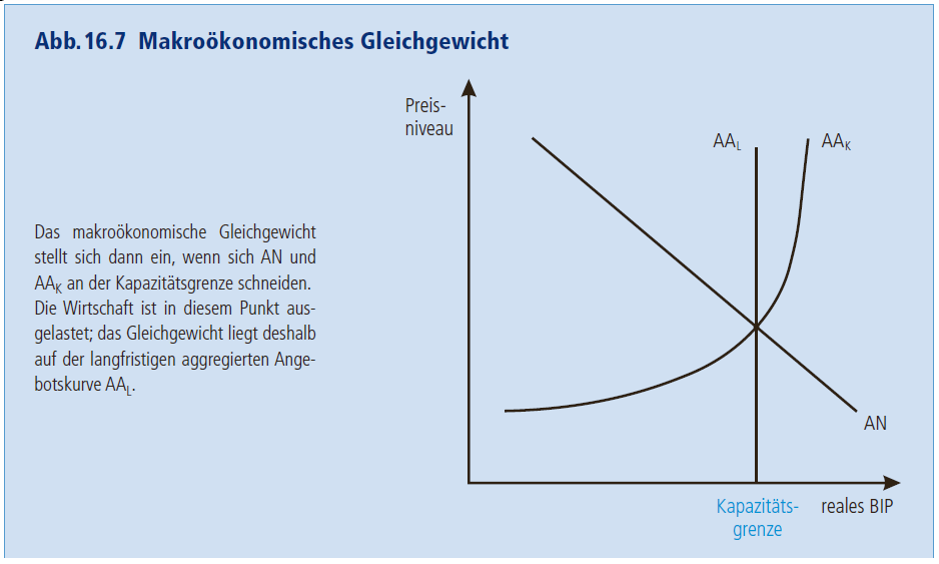
\includegraphics[width=12cm]{images/makro.png}
\end{minipage}


	\subsubsection{aggregierte Nachfrage $AN$}
	Nachfrage nach Gütern (Waren und Dienstleistung) durch die vier volkswirtschaftlichen Akteure.
	\begin{itemize}
		\item Haushalt $\rightarrow$ Konsum
		\item Unternehmen $\rightarrow$ Investitionen
		\item Staat $\rightarrow$ Staatsausgaben
		\item Ausland $\rightarrow$ Nettoexporte = Exporte - Importe
	\end{itemize}
	\subsubsection{langfristig aggregiertes Angebot $AA_L$}
	Beziehung zwischen Produktionsfaktoren. Die Kapazitätsgrenze ist unabhängig vom Preisniveau.
	\begin{itemize}
		\item Arbeit
		\item Kapital
		\item Technologie
		\item Boden und Ressourcen
	\end{itemize}
	\subsubsection{kurzfristig aggregiertes Angebot $AA_K$}
	An der Kapazitätsgrenze sind die Produktionsfaktoren optimal, aber nicht maximal ausgelastet. Durch Überstunden und maximale Auslastung der Infrastruktur kann die $AA_K$-Kurve über der Kapazitätsgrenze liegen.
\clearpage
\pagebreak
\subsection{Bruttoinlandprodukt (BIP)}
\begin{center}
    Das Bruttoinlandprodult gibt den Gesamtwert aller Güter (Produkte und Dienstleistungen), welche innerhalb eines Jahres innerhalb der Grenzen der Volkswirtschaft hergestellt wurden abzüglich der notwendigen Vorleistungen.
\end{center}
Das Bruttonationaleinkommen wird aufgrund der erbrachten Leistungen des Staatsangehörigen \textbf{unabhängig} der Grenzen errechnet.
\begin{itemize}
	\item Das nominale BIP gibt die Wertschöpfung zu Marktpreisen an.
	\item Das reale BIP gibt die Wertschöpfung inflationsbereinigt an.
	\item Das reale BIP der Schweiz beträgt \textbf{ca. 645 Mia.} Franken.
\end{itemize}
\vspace{0.5cm}
Je höher das Bruttoinlandpordukt desto höher ist die  Lebensqualität und der soziale Fortschritt eines Landes. Hier ist zu erwähnen das bei armen Ländern ein geringes Wachstum zu spürbaren Anstieg der Lebensqualität führt. Um das BIP zu analysieren gibt es drei Ansätze
\begin{itemize}
	\item Produktionsansatz: Wertschöpfung der Wirschaftsakteure
	\item Einkommensansatz: Bezahlung der Produktionsfaktoren
	\item Verwendungsansatz: Wirtschaftssubjekte ihr Einkommen verwenden
\end{itemize}
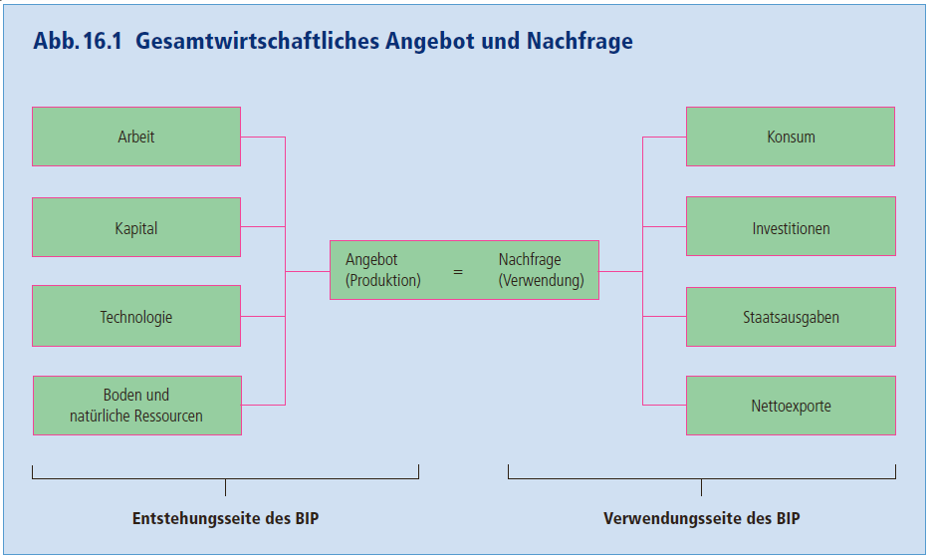
\includegraphics[width=0.8\linewidth]{images/bip.png}
\clearpage
\pagebreak
\section{Verteilung}
\subsection{Effizienz}
Pareto-Effizienz: Eine wirtschaftspolitische Massnahme ist dann effizient wenn sie die Situation eines Einzelnen verbessert, ohne andere schlechter zu stellen. 
\subsection{Verteilung}
\begin{itemize}
	\item Die Einkommensverteilung hängt ab von der Produktivität der Arbeitenden.
	\subitem Daher verdienen weniger leistungsfähige wenig.
	\item Will die Gesellschaft dies nicht akzeptieren, so muss umverteilt werden.
	\item Wird zu viel umverteilt gibt es weniger Anreize zur persönlichen Leistung.
	\item Wird zu wenig umverteilt wird dies als ungerecht empfunden.
	\item Die Herausforderung ist die Verteilung mit möglichst geringen Anreizen zur Verschwendung von Ressourcen zu erreichen
	\item Gini-Koeffizient sagt nichts über Wohlstand aus, sondern nur über die Einkommensverteilung
\end{itemize}
\begin{minipage}{0.7\linewidth}
    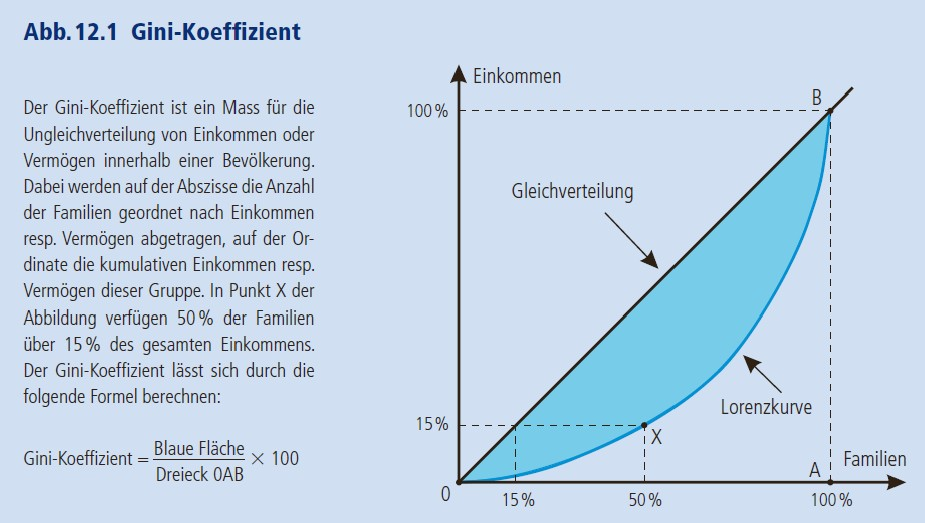
\includegraphics[width=\linewidth]{images/gini.jpg}
\end{minipage}
\begin{minipage}{0.3\linewidth}
    Je grösser der Gini-Koeffizient, um so schlechter / unfairer ist die Einkommensverteilung.
\end{minipage}
\subsection{Umverteilung} 
\begin{minipage}{5cm}
	\textbf{Einkommensquellen}
	\begin{itemize}
		\item Lohn
		\item Erträge aus Vermögen
		\item Staatliche Transfers
	\end{itemize}
\end{minipage}
\begin{minipage}{15cm}
	\textbf{Arten der Umverteilung}
	\begin{itemize}
		\item Umverteilung Einnahmen durch progressives Steuersystem (Einnahmeseite)
		\item Direkte Geldzahlungen (Ausgabeseite)
		\item Verbilligung staatliche Leistungen (Ausgabeseite)
	\end{itemize}
\end{minipage}
\clearpage
\pagebreak
\subsection{Umverteilung Ausgabenseite: Sozialwerke}
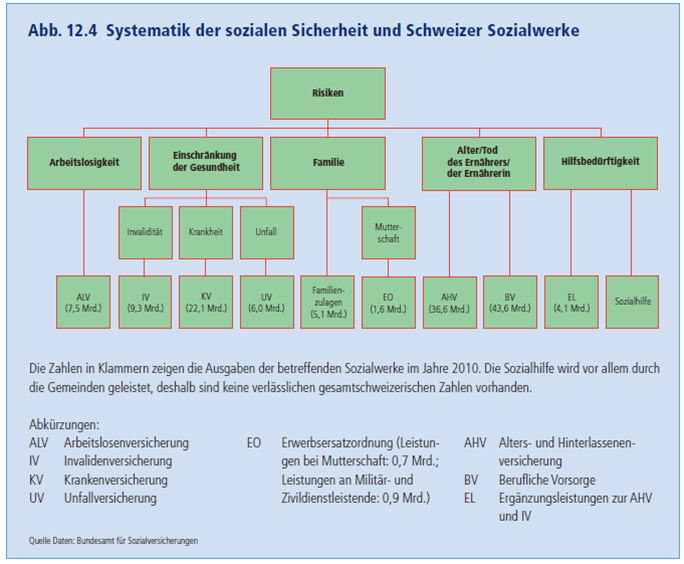
\includegraphics[width=0.8\linewidth]{images/sozialwerke.png}
\subsection{Die drei Säulen der Altersvorsorge der Schweiz}
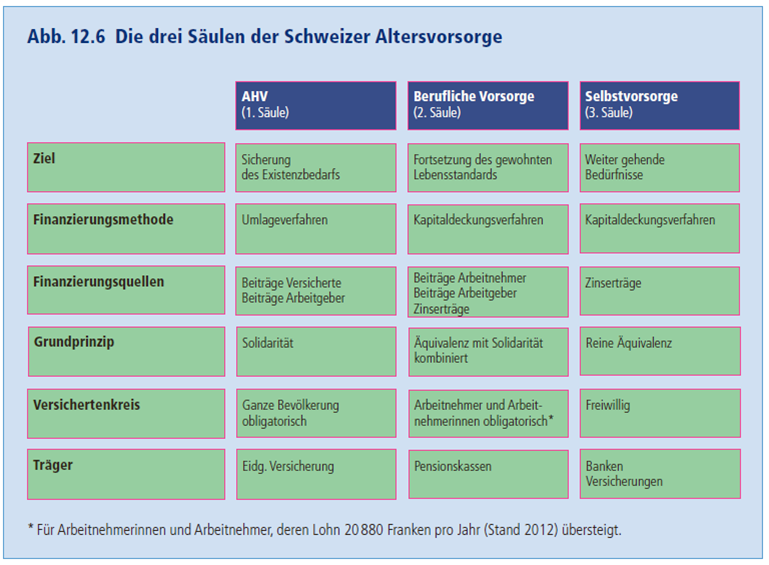
\includegraphics[width=0.8\linewidth]{images/dreissaulen.png}
\clearpage
\pagebreak
\section{Wachstum}
\subsection{Langfristiger Wachstumstrend}
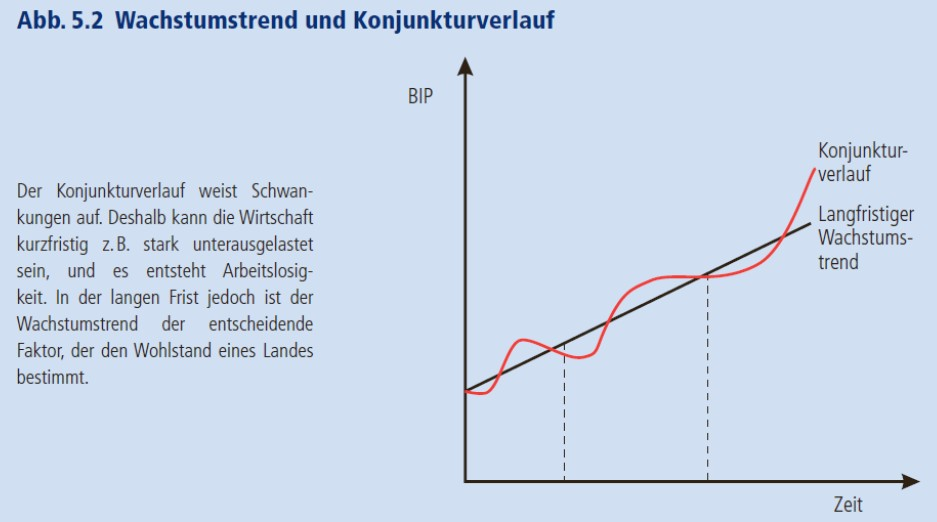
\includegraphics[width=0.7\linewidth]{images/wachstum.jpg}
\subsection{Quellen des Wachstums}
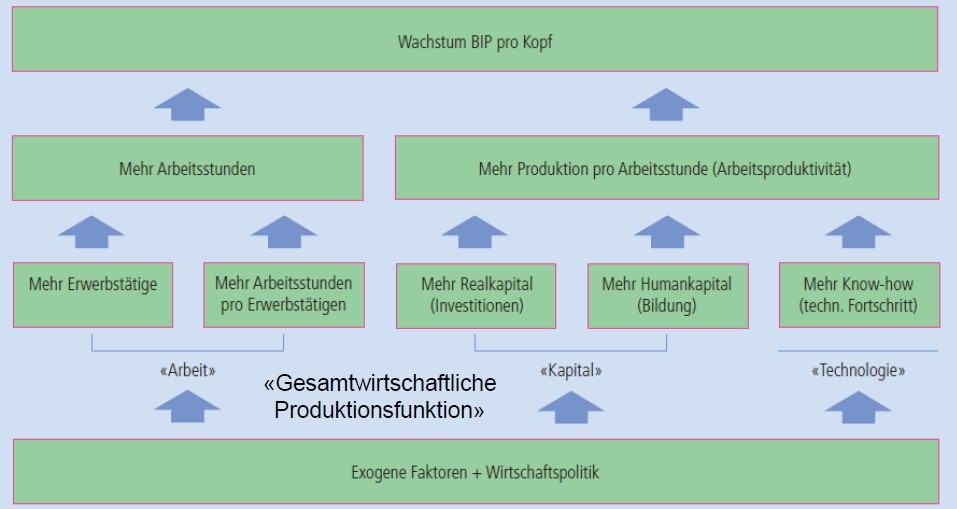
\includegraphics[width=0.7\linewidth]{images/quellen.jpg}
\subsubsection{Exogene Faktoren}
\begin{itemize}
	\item Ausstattung mir Rohstoffen
	\item Klima
	\item Nähe zu Handelspartnern
	\item Sozialkapital
	\subitem politische Stabilität
	\subitem Ausgestaltung der politischen Rechte
	\subitem Vertrauen in Eigentums- und Vertragsrechte
	\subitem tiefe Korruption
\end{itemize}
\begin{multicols}{2}
\subsubsection{Schweizer Wachstumssflaute}
\begin{itemize}
	\item Problem der Schweizer Hochpreisinsel (Abschottung Binnenmarkt)
	\item Höheres Wachstum der Schweizer Staatsquote
	\item Nicht schuld ist die höhere Immigration
\end{itemize}
\subsubsection{Staatsquote}
\begin{itemize}
	\item Staatsquote = (öffentliche Konsum + öffentliche Investitionen) / nominales BIP
	\item Zunehmender staatsnaher Sektor (Erziehung, Gesundheit, Soziale und Energie) expandiert und wirkt als Bremse für das Wachstum
\end{itemize}
\end{multicols}
\section{Arbeitsmarkt}
\begin{itemize}
	\item Arbeitslosigkeit existiert dann, wenn Haushalte bereit sind zum Marktlohn Arbeit anzubieten, diese aber nicht vom Unternehmen nachgefragt werden.
	\item Keine Arbeitslosigkeit herrscht dann, wenn Haushalte den Marktlohn als zu tief empfinden und deshalb keine Arbeit anbieten.
\end{itemize}
Zwei Typen der Arbeitslosigkeit\\
\begin{minipage}{12cm}
	\begin{itemize}
		\item \textbf{Sockelarbeitslosigkeit (X)}
		\item Anzahl der offenen Stellen ist gleich oder grösser als die Anzahl der Arbeitslosen (strukturelle und friktionelle Arbeitslosigkeit)
		\item \textbf{Konjukturelle Arbeitslosigkeit (Y)}
		\item Anzahl der Arbeitslosen ist grösser als Anzahl der offenen Stellen
	\end{itemize}
\end{minipage}
\begin{minipage}{5cm}
	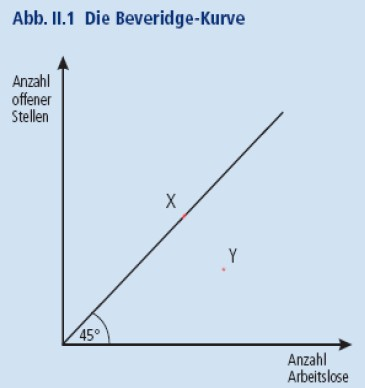
\includegraphics[width=4cm]{images/beveridge.jpg}
\end{minipage}
\subsection{Messung der Arbeitslosigkeit}
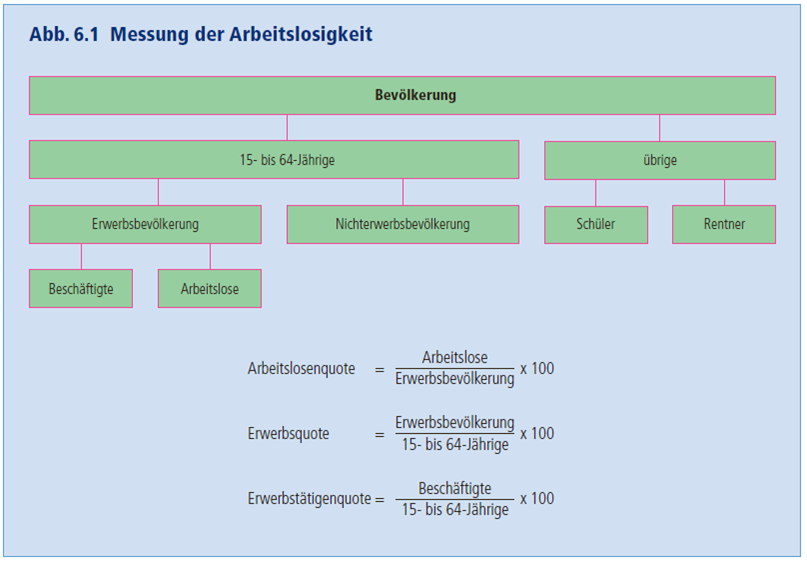
\includegraphics[width=0.8\linewidth]{images/messung.png}
\subsection{Der flexible Arbeitsmarkt}
\begin{multicols}{2}
	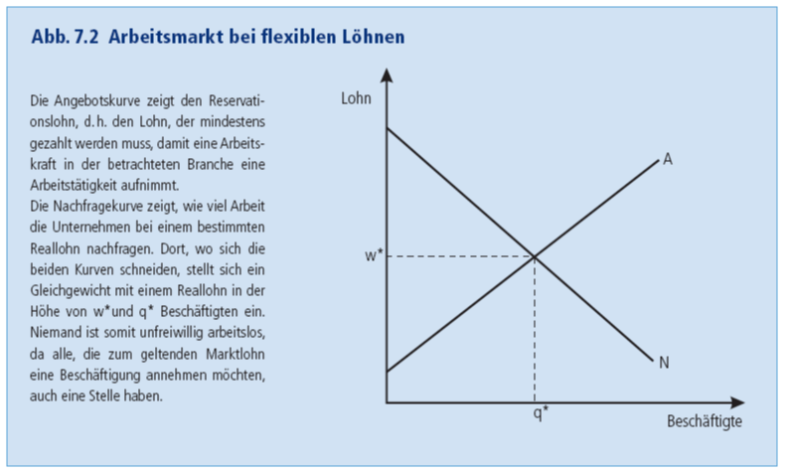
\includegraphics[width=0.95\linewidth]{images/felxibellohne.png}
	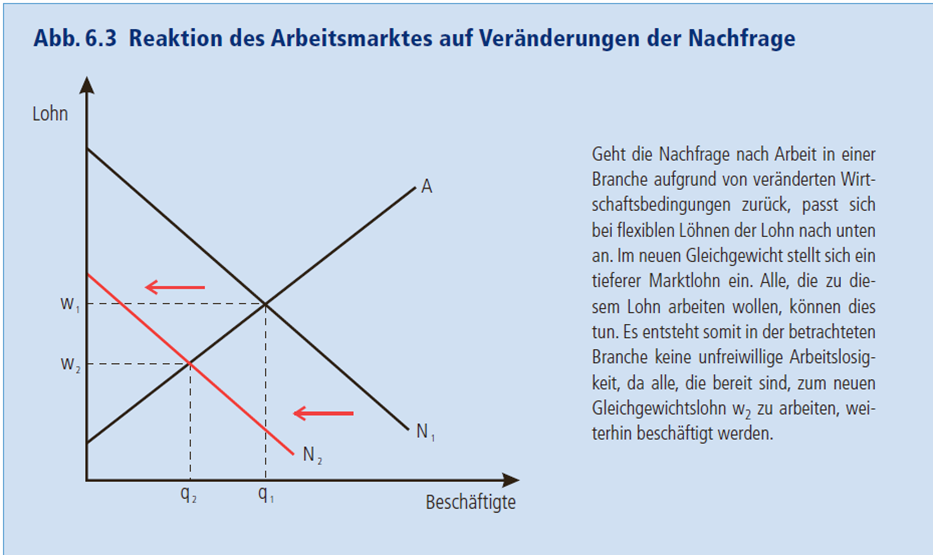
\includegraphics[width=0.95\linewidth]{images/flexibellohne2.png}
\end{multicols}
\subsection{Der regulierte Arbeitsmarkt}
	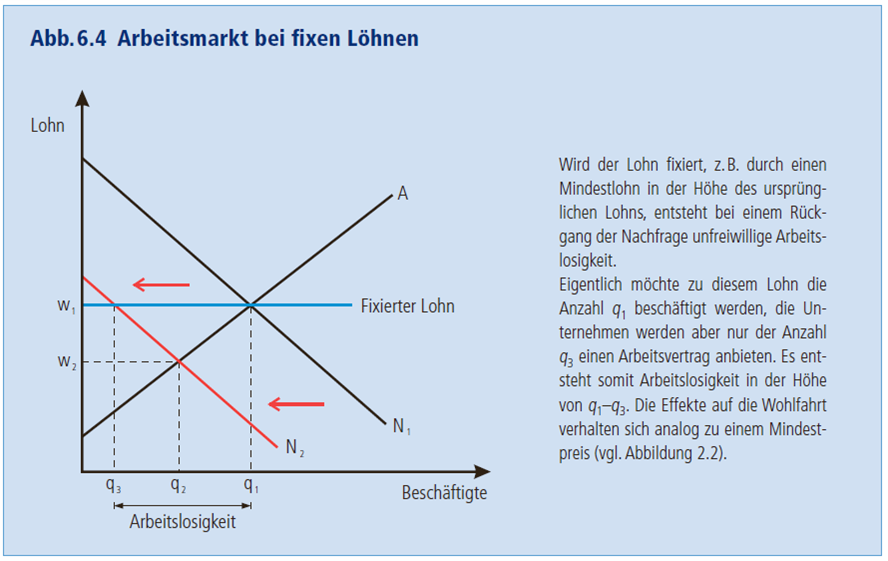
\includegraphics[width=0.8\linewidth]{images/fixelohne.png}

	\subsection{Sockelarbeitslosigkeit}
	\begin{itemize}
		\item \textbf{Strukturelle}
		\subitem Mindestlöhne
		\subitem Zentralisierte Lohnverhandlungen
		\subitem Regulierungen der Anstellung/Entlassung
		\subitem Regulierungen der Arbeitszeit
		\subitem Ausgestaltung der Arbeitslosenversicherung (Bezugshöhe)
		\item \textbf{Friktionelle}
		\subitem Ausgestaltung Arbeitslosigkeit (Bezugsdauer)
		\subitem Zeitspanne zum Finden einer neuen Stelle
	\end{itemize}
	\subsection{Arbeitsmarktpolitik der Schweiz}
	Die Schweiz hat eine sehr kleine Regulierungsdichte, Frankreich hat eine sehr hohe Regulierungsdichte und dadurch eine hohe Arbeitslosigkeit. Freie Arbeitsmärkte erholen sich sehr schnell. 
	\begin{enumerate}
		\item Mindestlöhne
		\subitem CH: Keine branchenübergreifende Mindestlöhne
		\item Zentralisierte Lohnverhandlungen
		\subitem CH: nur dezentral auf Branchenebene
		\item Regulierungen bezüglich Anstellungen und Entlassunge
		\subitem CH: wenig
		\item Ausgestaltung der Arbeitslosenversicherung
		\subitem CH: setzt auf Wiedereingliederung
		\item Regulierung der Arbeitszeit
		\subitem CH: wenig
	\end{enumerate}
\clearpage
\pagebreak



\section{Konjunktur}
\subsection{Der negative Nachfrageschock}
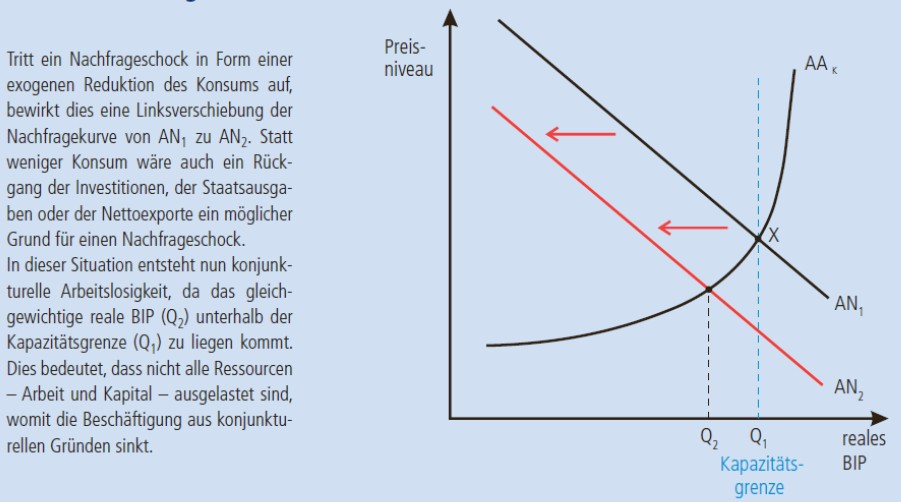
\includegraphics[width=0.8\linewidth]{images/negnach.jpg}
\begin{multicols}{2}
\subsection{Der kurzfristige positive Nachfrageschock}
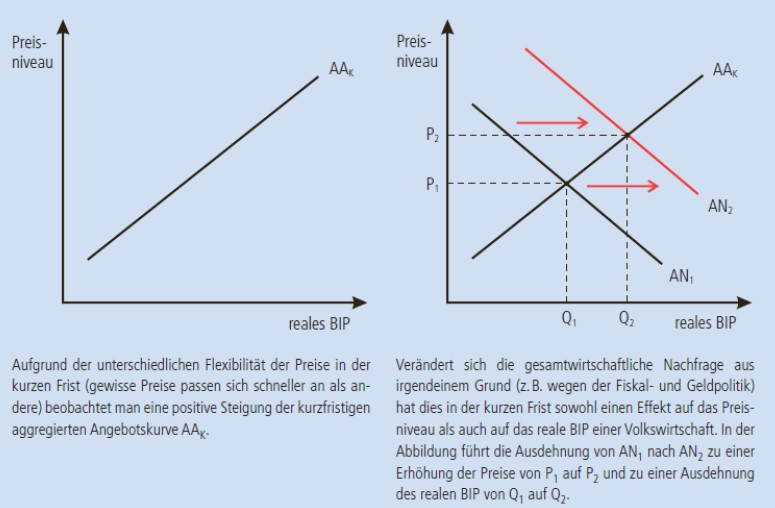
\includegraphics[width=0.98\linewidth]{images/posnachkurz.jpg}
\subsection{Der langfristige positive Nachfrageschock}
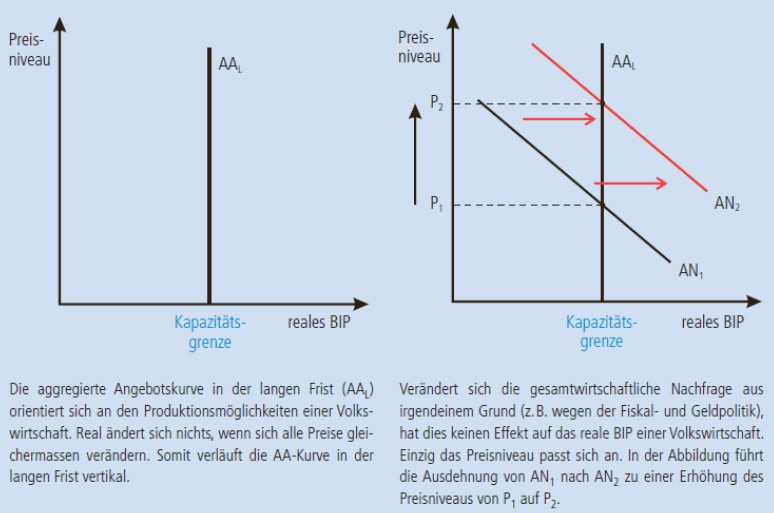
\includegraphics[width=0.98\linewidth]{images/posnachlang.jpg}
\end{multicols}
\begin{multicols}{2}
\subsection{Der negative Angebotsschock}
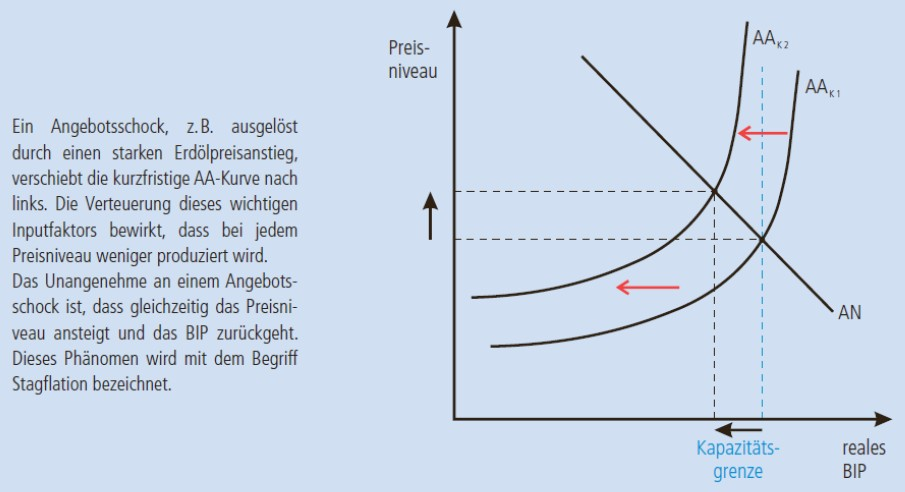
\includegraphics[width=0.98\linewidth]{images/negangebot.jpg}
\subsection{Der positive Angebotsschock}
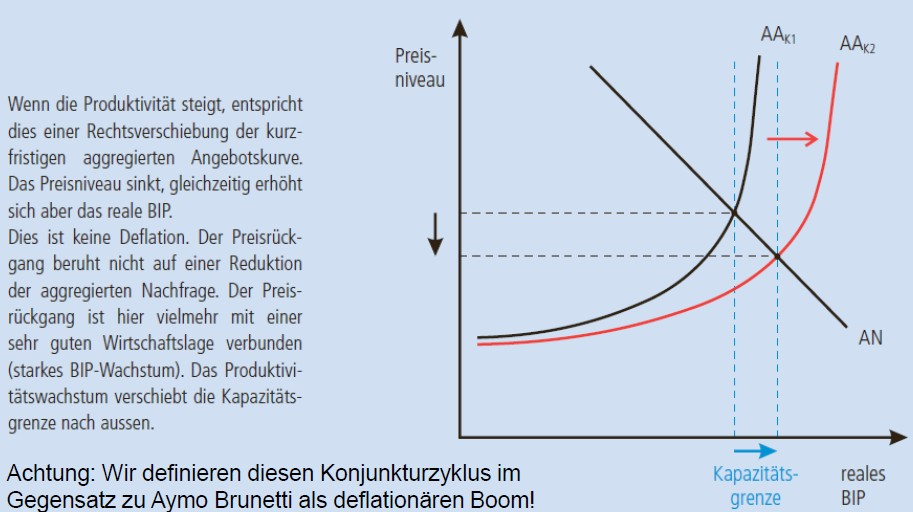
\includegraphics[width=0.98\linewidth]{images/posangebot.jpg}
\end{multicols}
\subsection{Konjunkturzyklen}
	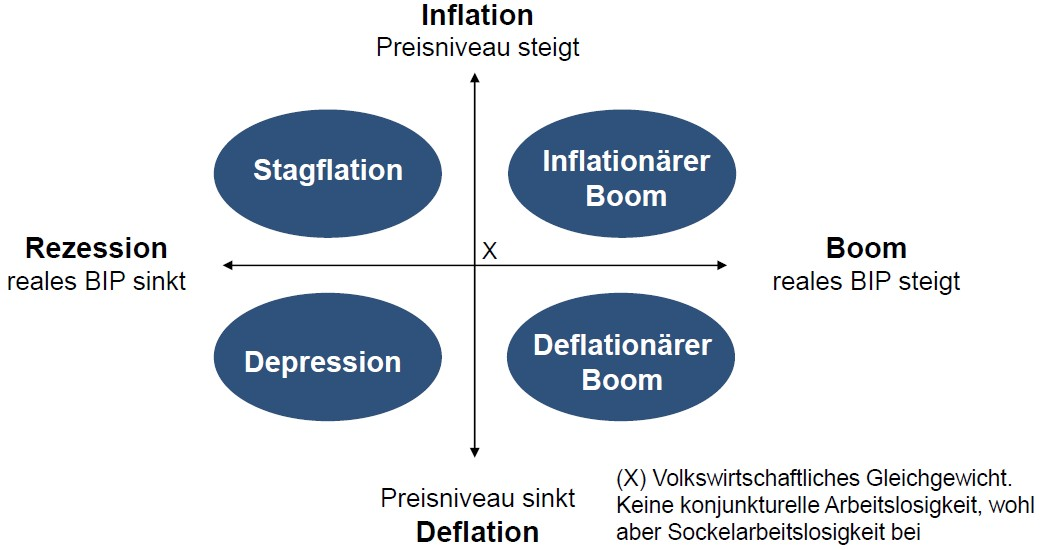
\includegraphics[width=15cm]{images/konjukturzyklen.jpg}\\
\begin{minipage}{10cm}
	\begin{itemize}
		\item \textbf{1.Nichts tun} 
		\subitem Anpassung ohne aktive Konjunkturpolitik
		\subitem Automatisches Wiederherstellen auf lange Sicht
		\subitem Zuerst Sinken der Löhne (Nominallöhne)
		\subitem Anschliessend tiefere Lohnkosten für Unternehmen dadurch höheres Angebot
		\subitem Gleiches BIP aber tieferes Preisniveau, tiefere Nominallöhne	
	\end{itemize}
\end{minipage}
\begin{minipage}{9cm}
	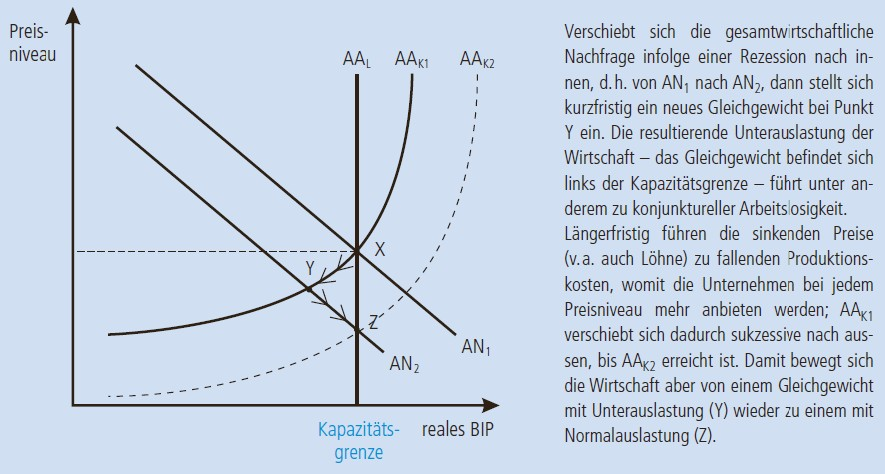
\includegraphics[width=9cm]{images/nichts.jpg}
\end{minipage}
\begin{minipage}{10cm}
	\begin{itemize}
		\item \textbf{2.Aktive keynesianische Konjukturpolitik}
		\subitem Märkte gehen von selbst, aber langsam wieder ins Gleichgewicht
		\subitem Positiver Schock auf Nachfrageseite
		\subitem Staat fördert durch Fiskal- und Geldpolitik Konsumnachfrage
		\subitem Staat erhöht Ausgaben
		\subitem Stimulierung der Investitionsnachfrage der Unternehmen durch tiefe Zinsen
		\subitem Erhöhung der Nettoexporte durch schwächere Währung (Erhöhung der Geldmenge)
		\subitem Problem der Wirkungsverzögerung
	\end{itemize}
\end{minipage}
\begin{minipage}{9cm}
	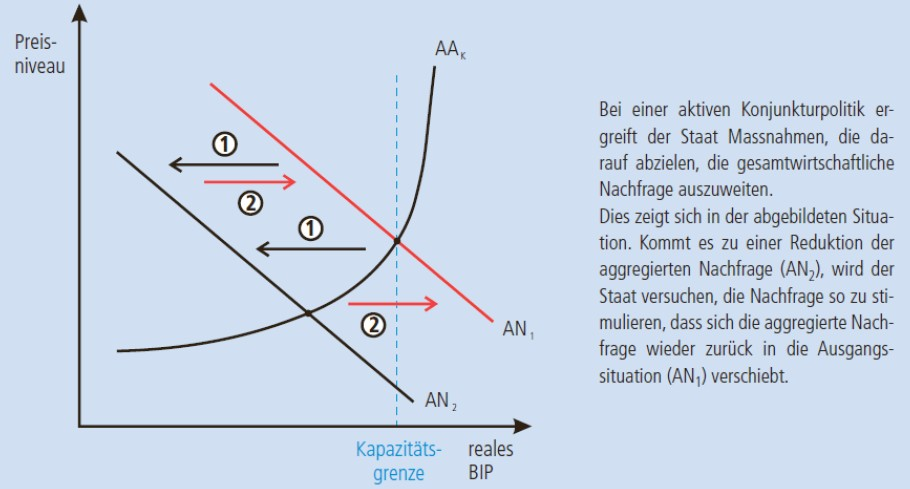
\includegraphics[width=9cm]{images/keyne.jpg}
\end{minipage}
\begin{minipage}{10cm}
	\begin{itemize}
		\item \textbf{3.Stärkung automatische Stabilisatoren}
		\subitem Staatliche Einnahmen und Ausgaben, dass automatisch Nachfrage stimuliert werden
		\subitem Steuern, Schuldenbremse, Arbeitslosenversicherung
	\end{itemize}
\end{minipage}
\begin{minipage}{9cm}
	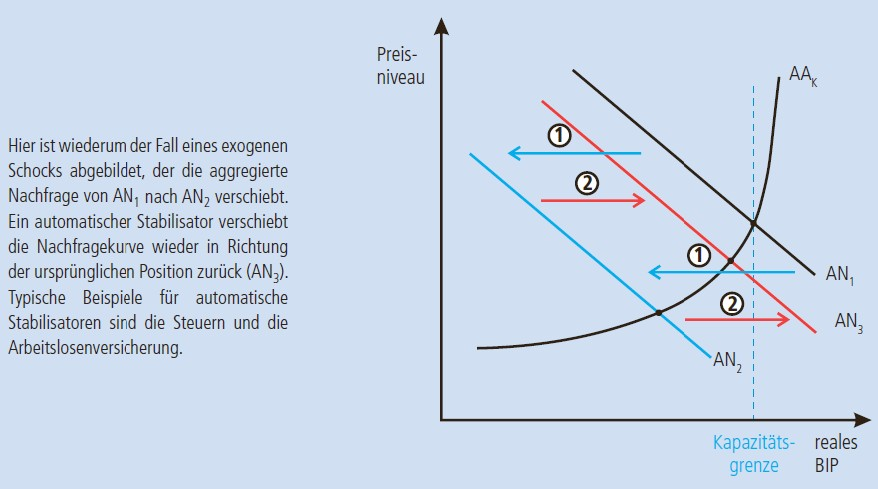
\includegraphics[width=9cm]{images/autostab.jpg}
\end{minipage}
\clearpage

\section{Preisstabilität}
\subsection{Inflation}
Eine Inflation bedeutet eine permanente Steigerung des Preisniveaus.\\
Auslöser ist eine einmalige Steigerung des Preisniveaus durch einen positiven Nachfrageschock oder einen negativen Angebotsschock. Ob dies zu einer Inflation führt hängt von der Inflationserwartung der Haushalte und Unternehmen. 
\subsubsection{Lohn-Preis-Spirale}
Erhöhtes Preisnivaeu durch einmaligen Schock
\begin{itemize}
	\item 1. Sinkende Reallöhne der Haushalte
	\item 2. Diese fordern (Inflationserwartung) eine Steigerung der Nominallöhne, welche die Erhöhung des Preisniveau überkompensiert
	\item 3. Damit ergbit sich eine Steigerung der Reallöhne
	\item 4. Dies bedeutet für die Unternehmen eine Kostensteigerung
	\item 5. Die Unternehmen werden deshalb höhere Güterpreise verlangen
	\item 6. Damit erhöht sich wieder das Preisniveau (Zweitrundeneffekt)
	\item Retour zu 1.
\end{itemize}
Die Inflation funktioniert nur, wenn die Nationalbank mitspielt und Geld druckt. Erwarten die Haushalte keine Steigerung setzt sich die Spirale nicht in Bewegung. 
\subsubsection{Quantitätsgleichung}
\begin{equation*}
	Preisniveau \cdot reales\quad BIP = Geldmenge \cdot Geldumlaufgeschwindigkeit \\
	P \cdot Q = M \cdot V
\end{equation*}
\subsection{Deflation}
Eine Deflation bedeutet ein permanenter Rückgang des Preisniveau. 
Die Deflation ist dann schädlich wenn diese auf einem Rückgang der aggregierten Nachfrage beruht. Ein Preisrückgang aufgrund einer Ausweitung des aggregierten Angebots führt zu keiner Deflation. Die Deflation ist kaum durch Geldpolitik und Fiskalpolitik zu lösen, weil alle erwarten dass es günstiger wird, daher hat die Ausweitung der Geldmenge keinen Effekt. 
\section{Geld}
\section{Wechselkurse}
\section{Staatsfinanzen}
\section{Banken}
Banken erwirtschaften ihren Gewinn durch: Kreditvergabe mit geliehenem Geld (Zinsdifferenzgeschäft), Kommissionsgeschäft (Vermögensverwaltung, Investmentbanking), Eigenhandel.
\begin{itemize}
	\item Finanzierung von Unternehmen: entweder direkte Finanzierung durch Aktien und Obligationen oder durch indirekte Finanzierung durch die Banken. Bei Beiden sind die Haushalte der Ursprung.
	\item Banken als Finanzintermediäre (Zwischenliegende)
	Sie vermitteln das Kapital zwischen den Anlegern (den Haushalten) und den Kreditnehmern. Sie lösen dabei drei Probleme: 
	\subitem 1. Transformation von Fristen
	\subitem 2. Breitstellen von Informationen (an Kreditgeber und Nehmer)
	\subitem 3. Verteilung des Risikos bei Kreditausfall
	\item Die Banken sind immer stark verschuldet 
\end{itemize}
\begin{figure*}[h]
	\centering
	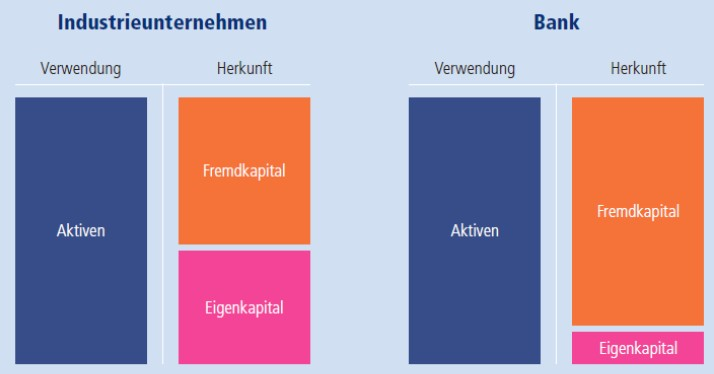
\includegraphics[width=0.7\linewidth]{images/banken.jpg}
\end{figure*}
\subsection{Risiken des Bankgeschäfts}
\begin{itemize}
	\item \textbf{Liquiditätsrisiko (Passivseite):} Falls die Kreditgeber (Haushalte) massenweise ihr Geld zurückfordern Bank-Run.
	\item \textbf{Solvenzrisiko (Aktivseite):}  Wenn die Bank auf der Aktivseite (verliehene Kredite) Verluste erleidet.Zum Beispiel bei Kreditausfällen oder Werteminderung der Wertpapieren. Diese Verluste müssen mit dem Eigenkapital gedeckt werden können. 
\end{itemize}
\subsection{Bankenregulierung}
Die Banken gehören zu den stärksten regulierten Branchen. Als Schutz für die Kunden und für die Stabilität des Finanzsystems.\\
\begin{minipage}{13cm}
	\begin{itemize}
		\item \textbf{Mikroprudentielle Regulierung (Stabilität einzelner Banken): } Aufgabe der FINMA-> kontrolliert Eigenkapital und Liquiditätsaustattung.
		\item \textbf{Makroprudentielle Regulierung (Stabilität des gesamten Bankensystems): }Aufgabe der SNB, sie setzt dabei auf Beobachtung und Entwicklung der Finanzmärkte (Prävention), wirkt bei den rechtlichen Rahmenbedingung mit und bietet eine Kurzfristige Vorsorge im Krisenfall.
	\end{itemize}
\end{minipage}
\begin{minipage}{6cm}
	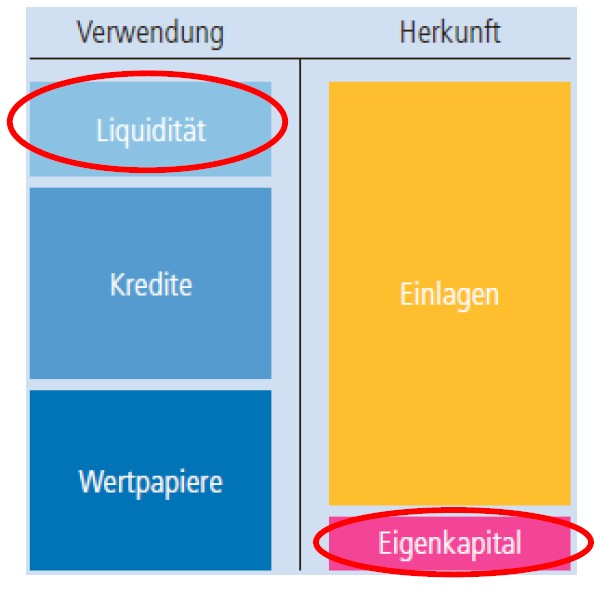
\includegraphics[width=6cm]{images/banken2.jpg}
\end{minipage}
\clearpage
\pagebreak
\subsubsection{Vorschriften}
\begin{itemize}
	\item Eigenkapitalvorschriften (Passivseite)
	\subitem Basel II (8\%) und Basel III (13\%)
	\item Liquiditätsvorschriften
	\subitem Obligatorische Einlageversicherung. Dies verhindert Bank-Runs, da der Kunde weiss, dass er sein Geld (bis zu einer definierten Obergrenze) trotz Liquiditätsproblemen der Bank zurück erhält.
	\subitem Liquiditätsvorgaben: Die Bank muss einen bestimmten Prozentsatz der Aktiven als flüssige Mittel
	halten. Dies ist für die Banken teuer (sie hat keine Erträge aus diesen Mitteln). Deshalb versuchen sich die Banken vor allem auf dem Geldmarkt bei anderen Banken zu finanzieren, da dieses Kapital in der Regel günstiger ist als das zur Verfügung gestellte Kapital der Haushalte.
	\item Makroprudentielle Vorschriften zur Konkursabwicklung
\end{itemize}
\subsubsection{Too Big to Fail}
Die gegenseitige kurzfristige Finanzierung von Banken in Form des Interbanken-Geschäfts (zwecks Liquiditätssicherung, aber teilweise auch für den Eigenhandel) führt zu einer starken Verflechtung des Bankensektors. Kommt es zu einem Bank-Run bei einer grossen Bank, können auch andere kreditgebende Banken unter Druck geraten.In einem solchen Fall müssen Zentralbanken bzw. Regierungen die insolventen Banken retten. Ein Scheitern dieser Banken würde unabsehbare Folgen für die Volkswirtschaft mit sich ziehen. Dies schafft eine unhaltbare Situation: die Banken werden ihre Risiken maximieren. Die Gewinne werden damit privatisiert, während die Allgemeinheit für die allfällige Verluste aufkommen muss (entspricht faktisch einer Staatsgarantie).\\
\textbf{Lösung dazu}\\
\begin{itemize}
	\item 1. Insolvenzverhinderung durch höhere Eigenkapitalforderung
	\item 2. Verfahren zur Konkursabwicklung beschrieben in Form eines living will (funktionsfähige Geschäftsbereiche abspalten)
\end{itemize}


\section{Die grosse Finanzkrise}
Nach 2001 verfolgte die USA eine sehr expansive Geldpolitik. Dadurch waren die Zinsen lange Zeit ungewöhnlich tief. Die tiefen Hypothekarzinsen verursachten ein rasches Ansteigen der Immobiliennachfrage und damit der Häuserpreise.
Gleichzeitig wurde ein innovatives Finanzinstrumentes kreiert –die ABS (asset-backed security) . Damit konnten neu Tausende von einzelnen Hypotheken gebündelt und in handelbare Wertpapiere verwandelt werden (Verbriefung). Die ABS wurden als risikolos (Triple-A) eingeschätzt und rentierten besser als vergleichbare Anlagen wie z.B. Staatsanleihen.
Damit floss viel Kapital in den US-amerikanischen Immobiliensektor, die Häuserpreise steigen unvermindert weiter und bildeten mit der Zeit eine eigentliche Finanzblase.
Schwächen in der Regulierung des US-amerikanischen Immobilienmarktes führten dazu, dass zunehmend auch an finanzschwache Haushalte grosszügige Immobilienkredite («Ninja-Kredite») vergeben wurden.
Kreditgeber wie auch Kreditnehmer spekulierten auf zukünftige Wertsteigerungen der gekauften Immobilie. Mit diesen Wertsteigerungen sollten die anfallenden Zinszahlungen beglichen werden.\\
Mitte 2006 begannen die Häuserpreise in den USA landesweit drastisch zu sinken. Gründe dazu waren. 
\begin{itemize}
	\item Ab 2004 hob die amerikanische Zentralbank schrittweise die Zinsen wieder an. Die Hypothekarzinsen der «Subprime»-Kredite stiegen dadurch rasch an.
	\item Die Immobiliennachfrage ging wegen den höheren Hypothekarzinsen zurück. Zudem mussten erste «Subprime»-Kreditnehmer ihre Immobilien an die Banken zurückgeben, weil sie die Zinsen nicht mehr bedienen konnten.
	\item Mit der zurückgehenden Nachfrage und dem steigenden Angebot nach Immobilien kamen die Häuserpreise rasch unter Druck. Die Banken reagierten mit einer vorsichtigeren Vergabe von Krediten (die Nachfragereduktion verstärkt sich dadurch).
	\item Die Preise der ABS sackten dadurch ins Bodenlose ab.
\end{itemize}
Dadurch wurde das Vertrauen in das internationale Bankensystem erschüttert. Die Zinsen im Interbankengeschäft stiegen stark und es wurde kein Geld mehr untereinander verliehen. Die Notenbanken mussten einspringen. 
\section{Markt und Preise}
\begin{itemize}
	\item Unbeschränkte Bedürfnisse stehen knappen Ressourcen gegenüber
	\item Wie wird das Budget auf unterschiedliche Verwendungszwecke aufgeteilt
	\item Opportunitätskosten: Kosten, die bei einer Entscheidung anfallen, dass die Vorteile einer Handlungsalternative nicht realisiert werden können
	\item Die Opportunitätskosten zeigen die Knappheit von Gütern in Form von Preisen an
	\item \textbf{Planwirtschaft}
	\subitem Ressourcen gehören Staat
	\subitem Staat lenkt Einsatz
	\item \textbf{Marktwirtschaft}
	\subitem Ressourcen gehören privaten Haushalten und Firmen 
	\subitem Private Haushalte/Firmen entscheiden über Ressourceneinsatz
	\subitem Preis spielt Hauptrolle
\end{itemize}
\subsection{Wirtschaftskreislauf}
\begin{multicols}{2}
	\subsubsection{Einfach}
	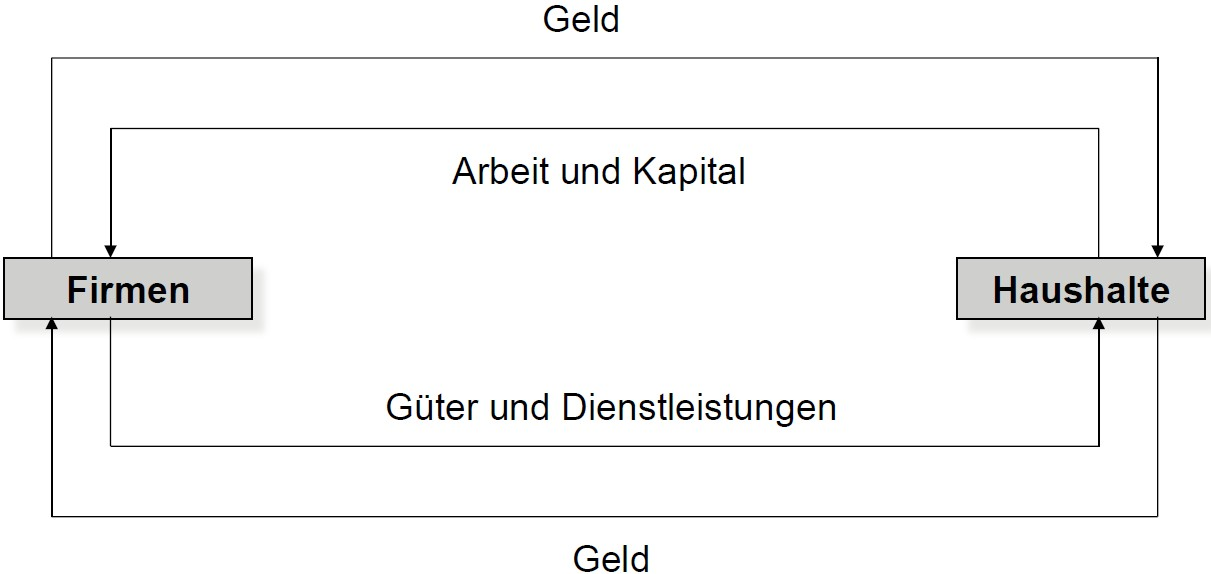
\includegraphics[width=9cm]{images/einfachWS.jpg}
	\subsubsection{Erweitert}
	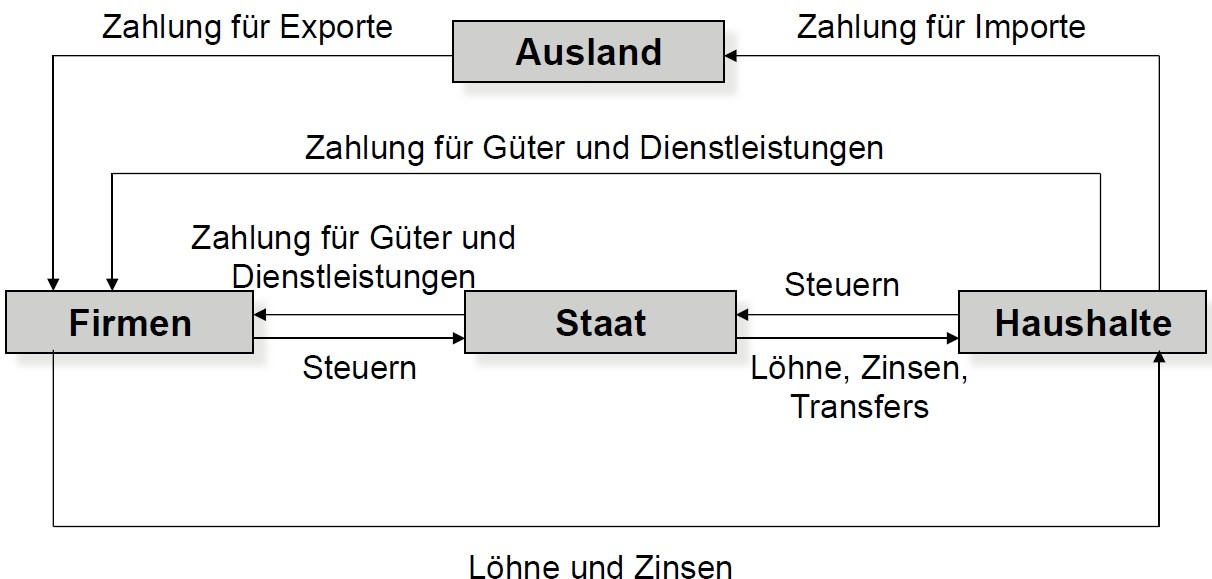
\includegraphics[width=9cm]{images/erweiterWS.jpg}
\end{multicols}
\subsubsection{Märkte}
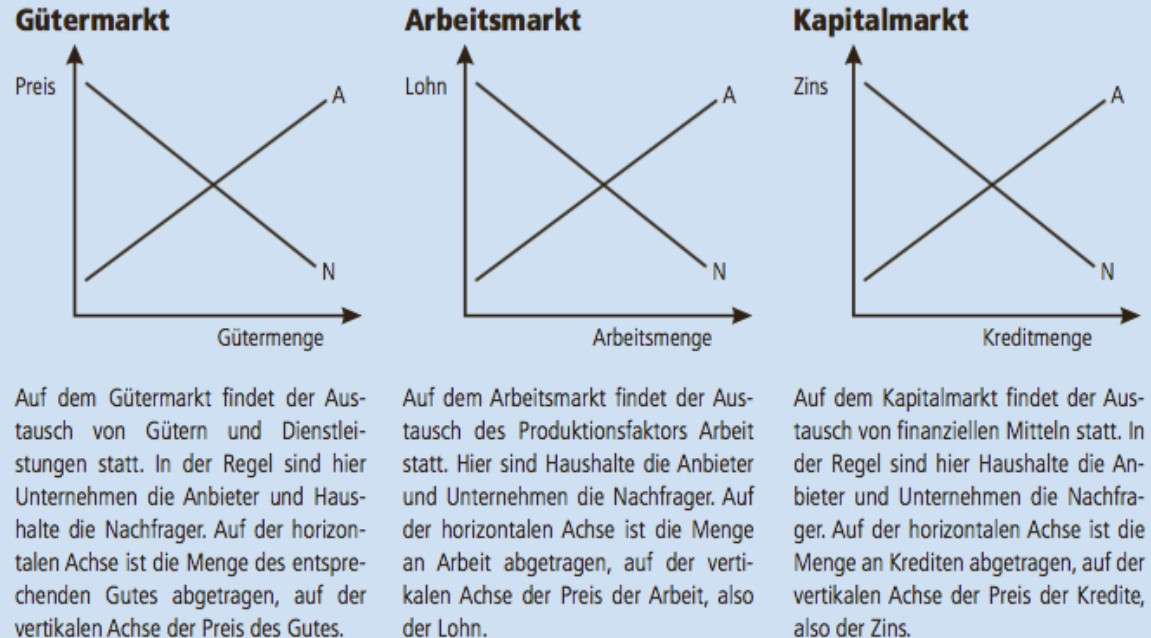
\includegraphics[width=15cm]{images/markte.jpg}
\clearpage
\pagebreak
\subsection{Mikroökonomisches Grundmodell}
\begin{itemize}
	\item Das Gut ist homogen
	\item Es gibt eine grosse Anzahl von Anbietern und Nachfragern
	\item Keine Marktzutrittshemmnisse
	\item Anbieter und Nachfrager sind über Mengen und Preise vollständig informiert
\end{itemize}
\begin{multicols}{2}
	\subsubsection{Konsumentenrente}
	Zahlungsbereitschaft des Käufers für ein Gut,
	abzüglich des Preises, den er tatsächlich dafür bezahlen muss\\
	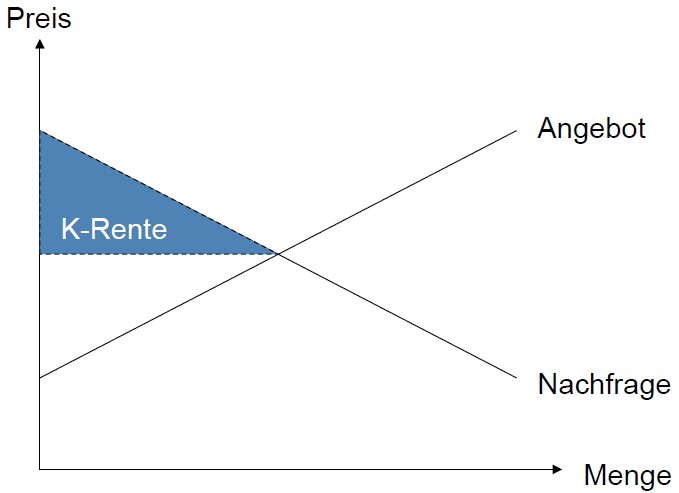
\includegraphics[width=7cm]{images/kr.jpg}
	\subsubsection{Produzentenrente}
	Erlös des Verkäufers für ein Gut, abzüglich der
	Kosten, die ihm für Erwerb oder Herstellung des Gutes entstanden sind\\
	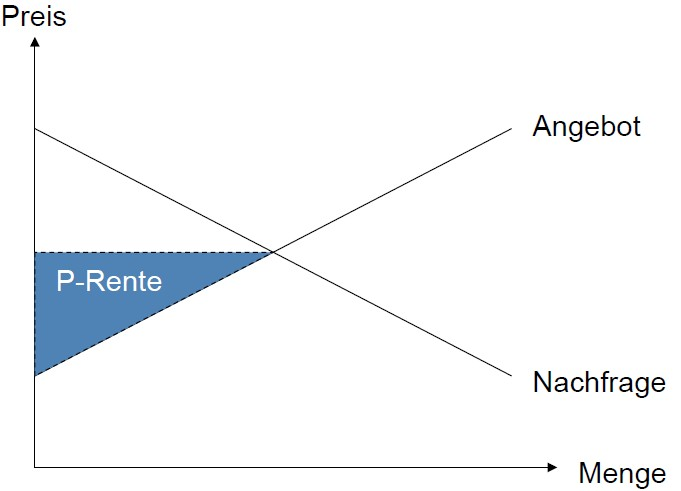
\includegraphics[width=7cm]{images/pr.jpg}
\end{multicols}
\subsubsection{Wohlfahrt}
Gesamte Rente, die auf einem Markt entsteht (Summe
aus Konsumenten- und Produzentenrente)
\begin{figure*}[h]
	\centering
	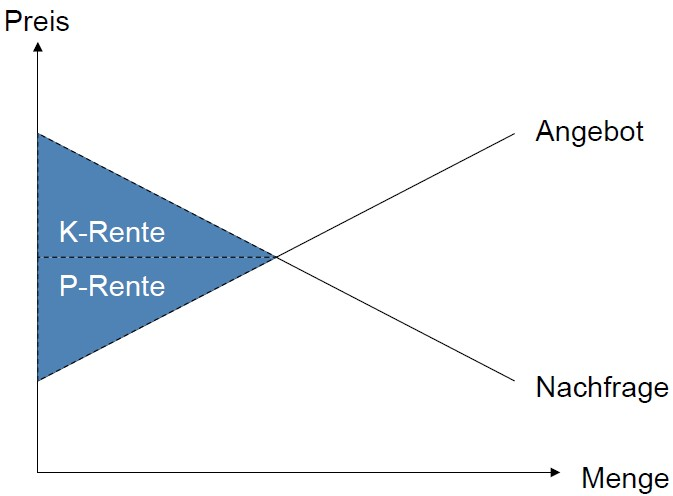
\includegraphics[width=6cm]{images/wohlfahrt.jpg}
\end{figure*}
\subsection{Preiseingriffe}
\begin{multicols}{2}
	\subsubsection{Mindestpreis}
	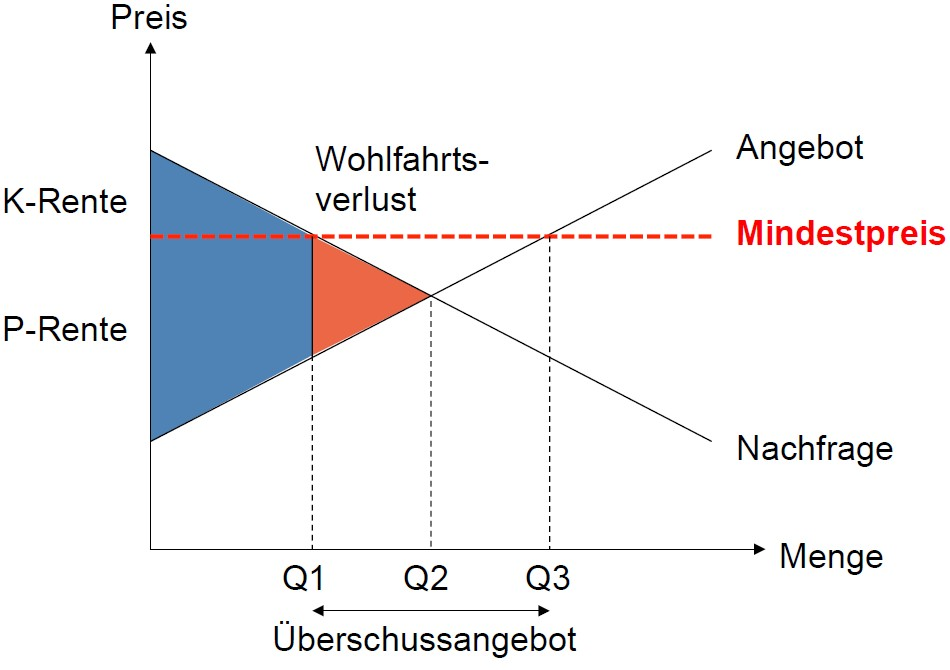
\includegraphics[width=7cm]{images/mindestpreis.jpg}
	\subsubsection{Höchspreis}
	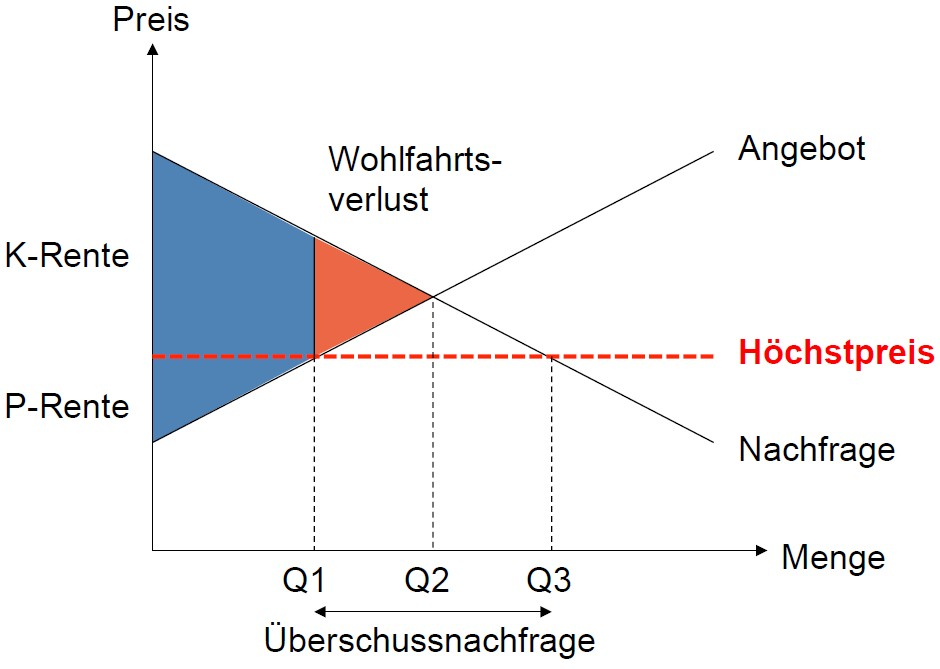
\includegraphics[width=7cm]{images/hochstpreis.jpg}
\end{multicols}


\section{Internationale Arbeitsteilung}
\subsection{Komparativer Kostenvorteil}
\begin{multicols}{2}
	Vorgehen:
	\begin{itemize}
		\item Opportunitätskosten Berechnen für alle Artikel.
		\item Opportunitätskosten vergleichen.
		\item Der Ort mit den tiefsten Opportunitätskosten produziert und
		exportiert zu einem Preis zwischen Opportunitätskosten im
		Exportort und den Opportunitätskosten im Importort (natürlich nur ohne
		Zölle, Transportkosten etc.).
	\end{itemize}
	Falls Gleichstand ist findet kein Handel statt.
	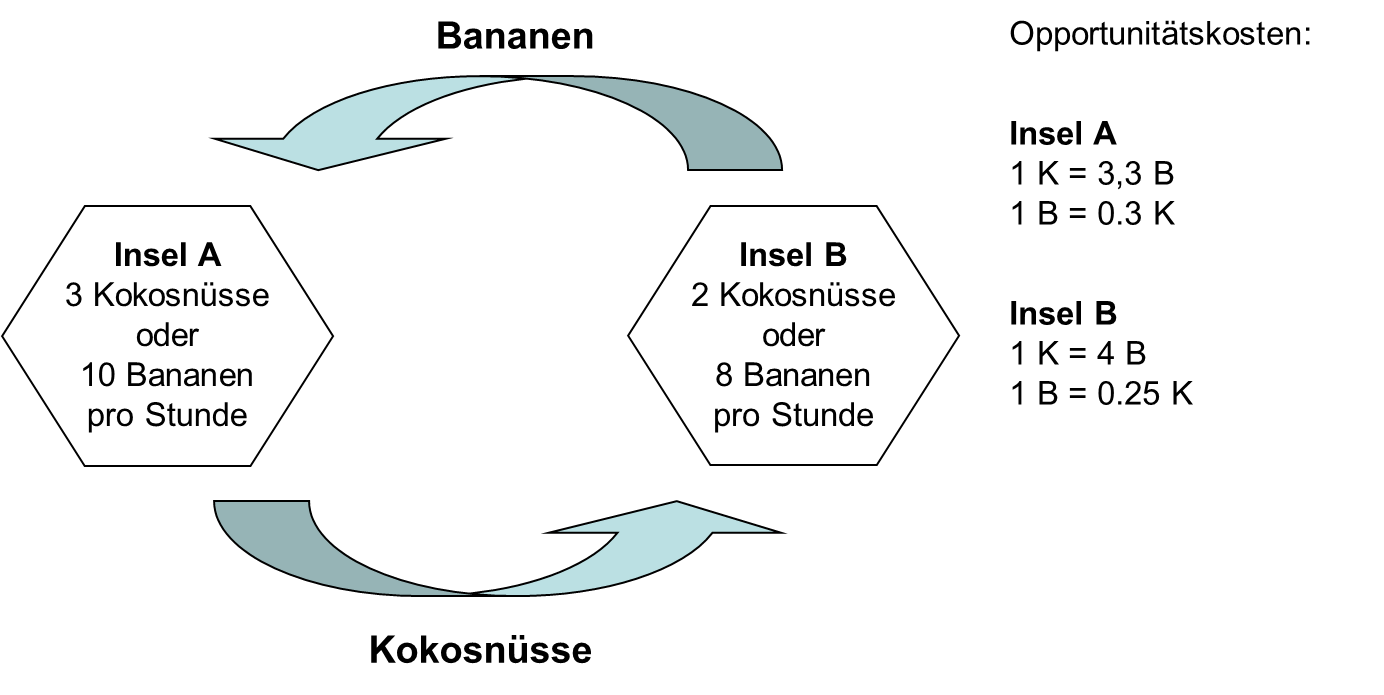
\includegraphics[width=9cm]{images/h03f07.png}
\end{multicols}
\subsection{Weltmarktpreis}
Hoher Weltmarktpreis: Konsument verliert, Allgemeinheit und Produktion gewinnt.\\
Tiefer Weltmarktpreis bewirkt genau das Gegenteil.\\
Internationale Arbeitsteilung bringt positive Wohlfahrtseffekte unabhängig
davon, ob der Weltmarktpreis höher oder tiefer als der Heimmarktpreis ist.
\begin{multicols}{2}
	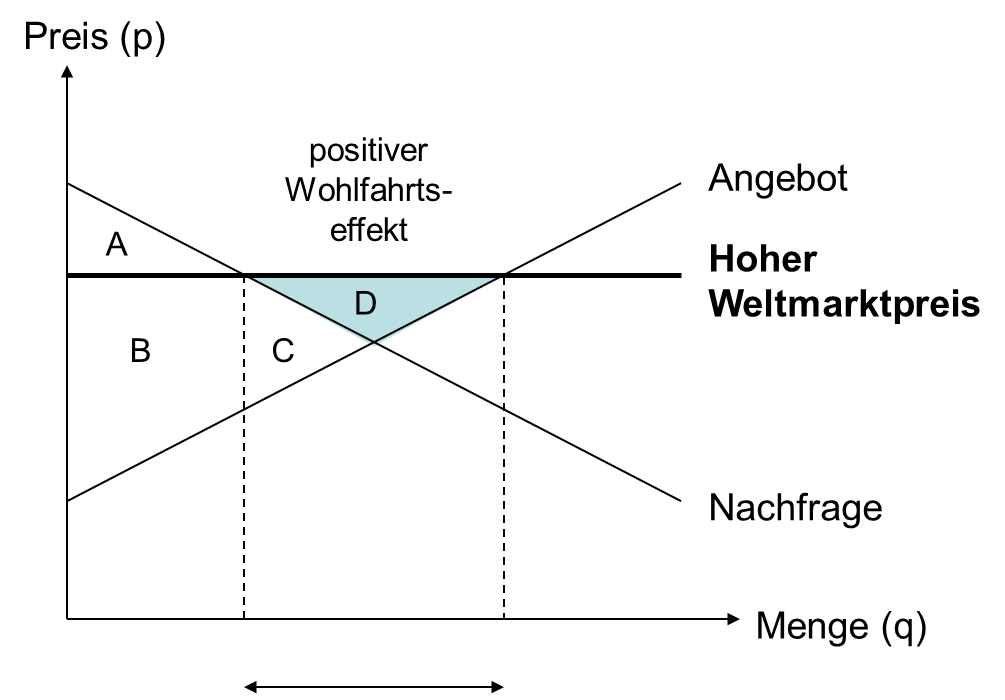
\includegraphics[width=9cm]{images/h03f11.png}\\
	\columnbreak\\
	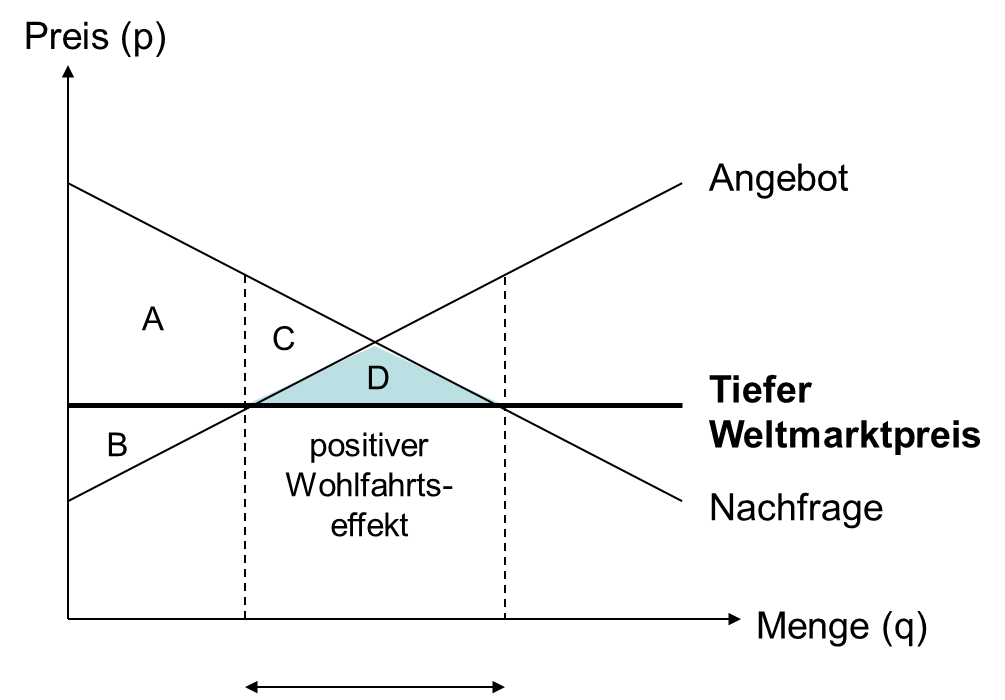
\includegraphics[width=9cm]{images/h03f13.png}
\end{multicols}
\subsection{Protektionismus (Zölle)}
\section{Europäische Integration}

\end{document}
